%%%%%%%%%%%%%%%%%%%%%%%%%%%%%%%%%%%%%%%%%
% Thesis 
% LaTeX Template
% Version 1.3 (21/12/12)
%
% This template has been downloaded from:
% http://www.latextemplates.com
%
% Original authors:
% Steven Gunn 
% http://users.ecs.soton.ac.uk/srg/softwaretools/document/templates/
% and
% Sunil Patel
% http://www.sunilpatel.co.uk/thesis-template/
%
% License:
% CC BY-NC-SA 3.0 (http://creativecommons.org/licenses/by-nc-sa/3.0/)
%
% Note:
% Make sure to edit document variables in the Thesis.cls file
%
%%%%%%%%%%%%%%%%%%%%%%%%%%%%%%%%%%%%%%%%%

%----------------------------------------------------------------------------------------
%	PACKAGES AND OTHER DOCUMENT CONFIGURATIONS
%----------------------------------------------------------------------------------------


\documentclass[11pt, a4paper, oneside]{Thesis} % Paper size, default font size and one-sided paper

\graphicspath{{./Pictures/}} % Specifies the directory where pictures are stored

\usepackage[utf8]{inputenc}
\usepackage[T1]{fontenc}
\usepackage[square, numbers, comma, sort&compress]{natbib} % Use the natbib reference package - read up on this to edit the reference style; if you want text (e.g. Smith et al., 2012) for the in-text references (instead of numbers), remove 'numbers' 
\usepackage{algpseudocode}
\usepackage{dirtree}
\usepackage{tikz}
\usepackage{pgfplots}
\hypersetup{urlcolor=black, colorlinks=false} % Colors hyperlinks in blue - change to black if annoying
\title{\ttitle} % Defines the thesis title - don't touch this

\begin{document}

\frontmatter% Use roman page numbering style (i, ii, iii, iv...) for the pre-content pages

\setstretch{1.3} % Line spacing of 1.3

% Define the page headers using the FancyHdr package and set up for one-sided printing
\fancyhead{} % Clears all page headers and footers
\rhead{\thepage} % Sets the right side header to show the page number
\lhead{} % Clears the left side page header

\pagestyle{fancy} % Finally, use the "fancy" page style to implement the FancyHdr headers

\newcommand{\HRule}{\rule{\linewidth}{0.5mm}} % New command to make the lines in the title page

% PDF meta-data
\hypersetup{pdftitle={\ttitle}}
\hypersetup{pdfsubject=\subjectname}
\hypersetup{pdfauthor=\authornames}
\hypersetup{pdfkeywords=\keywordnames}

%----------------------------------------------------------------------------------------
%	TITLE PAGE
%----------------------------------------------------------------------------------------

\begin{titlepage}
\begin{center}

\textsc{\LARGE \univname}\\[1.5cm] % University name
\textsc{\Large Master Thesis}\\[0.5cm] % Thesis type

\HRule \\[0.4cm] % Horizontal line
{\huge \bfseries \ttitle}\\[0.4cm] % Thesis title
\HRule \\[1.5cm] % Horizontal line
 
\begin{minipage}{0.4\textwidth}
\begin{flushleft} \large
\emph{Author:}\\
{\authornames} % Author name - remove the \href bracket to remove the link
\end{flushleft}
\end{minipage}
\begin{minipage}{0.4\textwidth}
\begin{flushright} \large
\emph{Supervisor:} \\
{\supname} % Supervisor name - remove the \href bracket to remove the link  
\end{flushright}
\end{minipage}\\[3cm]
 
\large \textit{A thesis submitted in fulfilment of the requirements\\ for the degree of \degreename}\\[0.3cm] % University requirement text
\textit{in the}\\[0.4cm]
\groupname\\\deptname\\[2cm] % Research group name and department name
 
{\large \today}\\[4cm] % Date
%\includegraphics{Logo} % University/department logo - uncomment to place it
 
\vfill
\end{center}

\end{titlepage}

%----------------------------------------------------------------------------------------
%	DECLARATION PAGE
%	Your institution may give you a different text to place here
%----------------------------------------------------------------------------------------

\Declaration{

\addtocontents{toc}{\vspace{1em}} % Add a gap in the Contents, for aesthetics

I, \authornames, declare that this thesis titled, '\ttitle' and the work presented in it are my own. I confirm that:

\begin{itemize} 
\item[\tiny{$\blacksquare$}] This work was done wholly or mainly while in candidature for a research degree at this University.
\item[\tiny{$\blacksquare$}] Where any part of this thesis has previously been submitted for a degree or any other qualification at this University or any other institution, this has been clearly stated.
\item[\tiny{$\blacksquare$}] Where I have consulted the published work of others, this is always clearly attributed.
\item[\tiny{$\blacksquare$}] Where I have quoted from the work of others, the source is always given. With the exception of such quotations, this thesis is entirely my own work.
\item[\tiny{$\blacksquare$}] I have acknowledged all main sources of help.
\item[\tiny{$\blacksquare$}] Where the thesis is based on work done by myself jointly with others, I have made clear exactly what was done by others and what I have contributed myself.\\
\end{itemize}
 
Signed:\\
\rule[1em]{25em}{0.5pt} % This prints a line for the signature
 
Date:\\
\rule[1em]{25em}{0.5pt} % This prints a line to write the date
}

\clearpage % Start a new page

%----------------------------------------------------------------------------------------
%	QUOTATION PAGE
%----------------------------------------------------------------------------------------

%\pagestyle{empty} % No headers or footers for the following pages

%\null\vfill % Add some space to move the quote down the page a bit

%\textit{``Thanks to my solid academic training, today I can write hundreds of words on virtually any topic without possessing a shred of information, which is how I got a good job in journalism."}

%\begin{flushright}
%Dave Barry
%\end{flushright}

%\vfill\vfill\vfill\vfill\vfill\vfill\null % Add some space at the bottom to position the quote just right

%\clearpage % Start a new page

%----------------------------------------------------------------------------------------
%	ABSTRACT PAGE
%----------------------------------------------------------------------------------------

\addtotoc{Abstract} % Add the "Abstract" page entry to the Contents

\abstract{\addtocontents{toc}{\vspace{1em}} % Add a gap in the Contents, for aesthetics

  Crawl.js aims at the practical importance of downloading pages efficiently and at high speed. The architecture is decentralized and workers are organized in groups (regions) which makes it locality-aware. Through the event-driven, non-blocking I/O model of Node.js\footnote{http://nodejs.org} the system is resource friendly and efficient. URLs are managed in redis\footnote{http://redis.io} sets and all operations are: asynchronous, atomic and able to handle multiple URLs (batch processing). Our combination of Node.js and redis showed a promising performance and scaling behaviour during our experiments.

}

\clearpage % Start a new page

%----------------------------------------------------------------------------------------
%	ACKNOWLEDGEMENTS
%----------------------------------------------------------------------------------------

\setstretch{1.3} % Reset the line-spacing to 1.3 for body text (if it has changed)

\acknowledgements{\addtocontents{toc}{\vspace{1em}} % Add a gap in the Contents, for aesthetics

  Especially I would like to thank {\supname } for giving me the opportunity to explore the domain of web crawlers and learn more about the novel JavaScript environment Node.js. Furthermore I'm grateful for the support of his team. Notably Pierre Sutra, who gave me the right papers to read and helped me reasoning about a huge performance bottleneck found during my experiments. Patrick Marlier, who kept complaints - a first buggy crawl caused - from me and who provided me the right profiling tools. All administrators involved who allowed me to use the powerful OpenNebula cluster hosted at the university. And last but not least I would like to thank all involved people for their patience. Especially my girlfriend who always supported me during my work.
}
\clearpage % Start a new page

%----------------------------------------------------------------------------------------
%	LIST OF CONTENTS/FIGURES/TABLES PAGES
%----------------------------------------------------------------------------------------

\pagestyle{fancy} % The page style headers have been "empty" all this time, now use the "fancy" headers as defined before to bring them back

\lhead{\emph{Contents}} % Set the left side page header to "Contents"
\tableofcontents % Write out the Table of Contents

\lhead{\emph{List of Figures}} % Set the left side page header to "List of Figures"
\listoffigures % Write out the List of Figures

%\lhead{\emph{List of Tables}} % Set the left side page header to "List of Tables"
%\listoftables % Write out the List of Tables

%----------------------------------------------------------------------------------------
%	ABBREVIATIONS
%----------------------------------------------------------------------------------------

\clearpage % Start a new page

\setstretch{1.5} % Set the line spacing to 1.5, this makes the following tables easier to read

\lhead{\emph{Abbreviations}} % Set the left side page header to "Abbreviations"
\listofsymbols{ll} % Include a list of Abbreviations (a table of two columns)
{
\textbf{URL} & \textbf{U}niform \textbf{R}esource \textbf{L}ocator \\
\textbf{Page} & A resource (typically html) identified by an \textbf{URL} \\
\textbf{Site} & A container for multiple pages. (ex. http://bs.wikipedia.org) \\
\textbf{VM} & \textbf{V}irtual \textbf{M}achine \\ 
}

%----------------------------------------------------------------------------------------
%	PHYSICAL CONSTANTS/OTHER DEFINITIONS
%----------------------------------------------------------------------------------------

%\clearpage % Start a new page

%\lhead{\emph{Physical Constants}} % Set the left side page header to "Physical Constants"

%\listofconstants{lrcl} % Include a list of Physical Constants (a four column table)
%{
%Speed of Light & $c$ & $=$ & $2.997\ 924\ 58\times10^{8}\ \mbox{ms}^{-\mbox{s}}$ (exact)\\
% Constant Name & Symbol & = & Constant Value (with units) \\
%}

%----------------------------------------------------------------------------------------
%	SYMBOLS
%----------------------------------------------------------------------------------------

%\clearpage % Start a new page

%\lhead{\emph{Symbols}} % Set the left side page header to "Symbols"

%\listofnomenclature{lll} % Include a list of Symbols (a three column table)
%{
%$a$ & distance & m \\
%$P$ & power & W (Js$^{-1}$) \\
% Symbol & Name & Unit \\

%& & \\ % Gap to separate the Roman symbols from the Greek

%$\omega$ & angular frequency & rads$^{-1}$ \\
% Symbol & Name & Unit \\
%}

%----------------------------------------------------------------------------------------
%	DEDICATION
%----------------------------------------------------------------------------------------

%\setstretch{1.3} % Return the line spacing back to 1.3

%\pagestyle{empty} % Page style needs to be empty for this page

%\dedicatory{For/Dedicated to/To my\ldots} % Dedication text

%\addtocontents{toc}{\vspace{2em}} % Add a gap in the Contents, for aesthetics

%----------------------------------------------------------------------------------------
%	THESIS CONTENT - CHAPTERS
%----------------------------------------------------------------------------------------

\mainmatter % Begin numeric (1,2,3...) page numbering

\pagestyle{fancy} % Return the page headers back to the "fancy" style

% Include the chapters of the thesis as separate files from the Chapters folder
% Uncomment the lines as you write the chapters

% Chapter Template

\chapter{Introduction} % Main chapter title

\label{Chapter1} % Change X to a consecutive number; for referencing this chapter elsewhere, use \ref{ChapterX}

\lhead{Chapter 1. \emph{Introduction}} % Change X to a consecutive number; this is for the header on each page - perhaps a shortened title

In this thesis we describe our approach of designing and implementing crawl.js. A distributed parallel web crawler written in node.js.
The goal..


\section{Node.js}

http://nodejs.org

\section{Outline}
In Chapter~\ref{Chapter2} we present the related work that has been done in this field and where crawl.js fits in.


% Chapter Template

\chapter{Related work} % Main chapter title

The research area of web crawling in general is big. In this thesis we want to focus on the work that has been done regarding architectures of web crawlers. Only a few have actually tried to build a scalable, parallel and distributed web crawler. The following sections present the different work that has been done organized by their idea.

\label{Chapter2} % Change X to a consecutive number; for referencing this chapter elsewhere, use \ref{ChapterX}

\lhead{Chapter 2. \emph{Related work}} % Change X to a consecutive number; this is for the header on each page - perhaps a shortened title

\section{Sequential crawlers}
One page is downloaded at the time. Nothing happens in parallel. Theses kind of web crawlers were used in the very beginning of the web. As the number of web pages grew the need to download web pages at a higher rate was obvious.


\section{Parallel crawlers}
\section{Centralized crawlers}
\section{Decentralized crawlers}

\subsection{UbiCrawler: a scalable fully distributed Web crawler \cite{ubicrawler}}

 
% Chapter Template
\chapter{Problem description} % Main chapter title
Building a slow crawler that runs on one machine and downloads several pages per minute is easy. Designing and implementing a distributed and parallel web crawler presents a number of challanges. In this chapter we want to discuss those more in detail.

\label{Chapter3} % Change X to a consecutive number; for referencing this chapter elsewhere, use \ref{ChapterX}

\lhead{Chapter 3. \emph{Problem description}} % Change X to a consecutive number; this is for the header on each page - perhaps a shortened title

\section{Size of the web}
Today (Thursday, 09 May, 2013) the size of the world wide web is at least 14.78 billion (10\textsuperscript{9}) indexed pages.\cite{wwwsize}

Here is a simple calculation to demonstrate how long it takes to download the entire web if you fetch one page after the other.
Lets assume an average page size of \textbf{320KB} \cite{webmetrics} (including resources such as images, scripts and stylesheets) and an ideal network connection of \textbf{100mbit/s}.

Based on these numbers it would take \textbf{~11.7 years}. And it becomes worse when you add a realistic latency of 100msec per page which adds another \textbf{~47 years} of idletime. So, in total it takes \textbf{58.7 years}.

As you can see, if you want to do download the web in a reasonable amout of time we have to \textbf{split} the work and \textbf{distribute} the parts so that we can do it in \textbf{parallel}.

\section{Split the work}
\subsection{Work splitting}
\subsection{Load balancing}

\section{Synchronization}
\subsection{Closeness}
\subsection{Politeness}



\chapter{Crawl.js} % Main chapter title
In this chapter we describe how crawl.js splits and distributes the work in detail.
\label{Chapter4} 
\lhead{Chapter 4. \emph{Crawl.js}} 

\section{System overview}
Crawl.js is a decentralized system. Each \emph{worker} in the system is standalone and autonomous and does not depend on any other worker. The only thing a worker needs is a connection to the \emph{Queues} and to the \emph{Stores}. Figure~\ref{system_overview} gives an overview of the main components in our system.

In order to explore our architecture, let us follow the path of an URL in the system.
The first thing a worker needs to do is get some URLs (Step 1) from a remote queue (Note that the worker knows by his own which Queue to ask). Steps 2 and 3 involves fetching, parsing and storing the content given by the URL. Thanks to the asynchronous nature (Streaming) of Crawl.js the parsing (Step 3) can happen before the fetching (Step 2) is completed. Even storing the content (Step 3) is done while fetching. Whenever a new URL is extracted in the parsing step it is added to the \emph{Queue}. The queue then decides what to do (Steps \emph{4a},\emph{4b}). Either it is kept in the local (in-memory) queue or dispatched to a remote one (batch processing).

\begin{figure}[h]
\centering
  \includegraphics[width=1\textwidth]{Figures/system_overview.pdf}
\caption{Crawl.js - System Overview}
\label{system_overview}
\end{figure}

\section{Mapper}
\label{mapper}
The mapper is not a physical component in the system like the \emph{Queue}, the \emph{Worker} or the \emph{Store}. It is a algorithm allowing each component at any time to map a URL to an identifier. This identifier is then used to determine the responsible \emph{Queue} or \emph{Store} for that URL.
This ability of being able to compute an identifier for a URL \emph{independently} is key to the whole system architecture. This ability is what makes the system decentralized. We do not have to ask a central component with manager like capabilities. We can compute the identifier ourself. Basically it identifies a virtual block within the URL space (all URLs). Every URL belongs to one and only one virtual block and each block is:
\begin{itemize}
  \item Mutual exclusive - Each block belongs to one and one worker only.
  \item Equally sized - From block to block the number of URLs should roughly be the same.
\end{itemize}

In other words the mapper is responsible to \emph{split} the work. In Crawl.js, the mapper is nothing more than a function implemented as a separate module. Each component that needs to be able to map a URL to an identifier just include the module. The algorithm used is rather simple and illustrated below:
\begin{algorithmic}[0]
\Function{Map}{$url$}\Comment{Map the URL to an identifier}
\State $host \gets url.host$\Comment{Only the host part ex. www.unine.ch}
\State $hash \gets \textbf{hash}(host)$\Comment{Hash the host part}
\State $id \gets hash \bmod n$\Comment{id $\in \{0,1,..n\}$, n:total number of virtual blocks}
\State \textbf{return} $id$
\EndFunction
\end{algorithmic}

So the idea is to hash the host part of the URL modulo the total number of blocks we want. The modulo number (total number of blocks) must be shared among every component using the mapper in the system.
To achieve this shared knowledge we can use a \emph{static} or a \emph{dynamic} approach. Using the static one is much simpler and achievable through simple configuration values. The key about the \emph{static} approach is that the number does not change during runtime. If we want to change the configuration, we have to shutdown all workers, reconfigure them and restart. Using the \emph{dynamic} approach would allow us to change the value while all workers continue to run. They would simply start mapping URLs to new identifiers as soon as we change the value. It is obvious that for the dynamic approach some sort of communication between the mappers is needed to interchange the newly assigned value of "total number of virtual URL blocks".

\subsection{Politeness}
To start, what does it mean for a crawler to be polite? There are different aspects of politeness like the robots exclusion protocol (discussed in \ref{worker}) that we do not want to discuss here. We want to discuss how often a crawler should access a server within a time frame. It is not especially the number (ex. once every 30 seconds) that is important but the fact that we need to be able to limit/control this number.

In order to do that we hash only the host part of the URL in our mapping function. Doing so guarantees that there is always only one worker responsible for one host\footnote{In our implementation we do not support the situation where several host names point to the same IP address (virtual hosts)}. Having this situation allows us now to control this aspect of politeness.
During our first test runs we accidentally hashed the whole URL. This resulted in an uncontrollable situation because multiple workers were fetching the same host simultaneously.

\subsection{Alternatives}
The introduced mapper function here is rather simplistic but because of its important role we built Crawl.js such that this component can easily be replaced. In the following we present an alternative mapper that we used throughout our experiments in Section~\ref{Chapter5}.

\subsection{2-level Mapper (Groups of workers)}
This novel mapper introduces the \emph{closeness} aspect. Closer sites should be crawled by workers near them (in terms of latency). 
\newline
As the name suggests it, the URL to worker assignment is done using 2 levels. The first level (e.g. hostname) determines the group and the second level (e.g. path + query part) identifies the worker within that group. The 2-level mapper introduces the notion of groups to Crawl.js which adds an additional dimension to the configuration. The number of groups and each group size can be configured independently. One group may have one worker and another three (e.g. depending on the number of URLs a group is responsible for).
\newline
With groups we have now the ability to configure Crawl.js in such a way that \emph{closeness} is respected. For example we can create a group \emph{region 1} responsible for crawling sites \emph{close} to that region. How different group configurations affect the total crawl performance will be shown in experiment 3.

\section{Queues}
Queues play a central role in the Crawl.js system. There are \emph{local} queues and \emph{remote} queues. Each worker keeps a local in-memory queue during his crawl for various reasons discussed in section \ref{queues_local} and each worker \emph{consumes} URLs from a remote queue. A remote queue represents one virtual URL block (as discussed in section \ref{mapper}). But, before we start with the details we state more precisely the term queue used in Crawl.js.

\subsection{Queue}
First a few words about how we use the word \emph{Queue} within this document. Strictly and technically speaking it is \emph{more} than a queue. A basic queue has the following operations:
\begin{itemize}
  \item enqueue
  \item dequeue
\end{itemize}

New items are enqueued at the bottom of the list and existing items are dequeued from the top. In terms of URLs this could work. But, what if we want to prioritize the URLs in the queue somehow. Of course we could enqueue URLs in the order we want them prioritized but this is rather inconvenient and does not work for existing URLs in the queue. We want to be able to re-prioritize (remove/change) existing URLs in the queue. As mentioned in \cite{hp_crawler}, fetching URLs in the order they were enqueued is a bad idea because of second-level locality in the links.

Therefore in Crawl.js a queue is a \emph{sorted set}. With sorted sets we can achieve whatever order we like. We can simulate a queue with it (that's why we still call it queue), use a pure random approach (set) or use custom algorithms to compute the order in the queues (re-visit policies).

\subsection{Consuming \& Producing}
The \emph{consumer} is the worker. Only one worker. Therefore, we need to assign each worker to the right remote queue which is done through a startup parameter. The parameter is not only the identifier of the queue but the identifier of the virtual URL block this worker is responsible for. We discussed the ability of every worker to be able to map an URL to an id in section \ref{mapper}. With the help of this additional parameter the worker can now decide if responsible for a given URL (compare the ids). If, the URL is added to the \emph{local} queue. Otherwise the URL is added to the appropriate \emph{remote} queue. Doing so makes the worker also a \emph{producer}. Obviously because there are multiple workers acting the same, we have a multiple producers situation for a single remote queue. 

\subsection{Local Queue (in-memory)}
\label{queues_local}
As the title describes it, from the worker's point of view it is a local and in-memory queue. The reason why every worker has a local queue is twofold:
\begin{itemize}
  \item We want the worker to be autonomous for a certain time. Therefore a place to put newly found URLs (during the crawl) is needed.
  \item Additionally we do not want to fetch the same URL twice (during one crawl of one worker). Therefore the local queue is the first filter used to eliminate duplicated URLs. Because the Queue is implemented as a sorted set, checking for the existence of an URL is easy and achievable with a O(1) complexity.
\end{itemize}

One thing to note is that the state of this local queue is in memory only. This means that when the worker crashes this state is lost. So we need to find a trade-off between autonomy and fault tolerance. We want the worker to be autonomous (no inter communication) as much as possible, but on the other side we do not want to lose much information if a worker crashes. Currently this trade off is adjustable with the help of a configuration value that limits the size of the queue. Once this limit is reached, the worker does not put any new URLs in the local queue but dispatches them to the \emph{remote} one so that the local queue is emptied and the crawl finished. An additional idea would be to limit a crawl in terms of time, but this is left as a future work.

\subsection{Remote Queue}
\label{queues_remote}
As mentioned in the introduction of this section, one worker is responsible for one queue but all other workers are able to fill it. The state of all remote queues represents the whole system state. URLs on the top of those queues are going to be fetched next and URLs at the bottom have just been fetched successfully. It is obvious that this state is important and needs to be persistent. 


\subsection{Remote Queue implementation (Redis.io)}
In Crawl.js remote queues are implemented with Redis\footnote{Redis - \url{http://www.redis.io}}. We use one sorted set for one remote queue. Hopefully, the sorted set from Redis gives us all the atomic operations we need. Redis uses the notion of score to sort the elements in the set. With the help of this score value we can, not only sort the elements within the queue, but also store the meta data associated to it. (ex. score > 0 := FETCHED, score < 0 := FETCH). Each element in the sorted set is a tuple <member, score> where the member is an URL in our case. How the worker uses the score together with the available commands is described below. Low (even negative) score values represent URLs that are going to be fetched next.

\begin{enumerate}
  \item \textbf{ZRANGEBYSCORE}\footnote{\url{http://redis.io/commands/zrangebyscore}} (single consumer) - get next URLs that need to be fetched. Note that the elements in the queue are not removed yet.
  \item \textbf{ZINCRBY} (multiple producers) - decrement the score of URL by a constant value. This happens when workers dispatch extracted URLs. It makes the entry move up the queue.
  \item \textbf{ZADD} (single producer) - As soon as an URL is fetched successfully we set the score to the current time stamp. This makes the entry move to the bottom of the queue.
\end{enumerate}

This is maybe not the best approach of how to prioritize URLs within the remote queues, but it was simple to implement and allowed us to run the first tests. The important thing to note here is that we have set a base with sorted sets that allows us to easily try out new approaches. As an example we could introduce an independent component in the system that takes care of computing the order of our queues based on some algorithms. (ex. Page rank).

\section{Stores}
Besides \emph{Queues} there is another important component in the system. \emph{Stores}. While queues persist the system state, stores persist the downloaded content (html, css, js, ..). The worker is able to identify his store using the \emph{mapper} module.
\subsection{Consuming \& Producing}
In this component we do not have \emph{consumers}, We have \emph{producers} only and because a worker is producing to his store only, there is no multiple producer situation for a single \emph{store}.

\subsection{Store}
The \emph{store} is here to persist the downloaded data of one worker. The API towards a store looks like this:
\begin{itemize}
  \item PUT (URL, DATA, [timestamp])
\end{itemize}
This abstraction gives us the ability to implement different store engines and encapsulate implementation details (batch-processing) in a modular way. Like the sorted sets in the queues, the store gives us the flexibility to do whatever we want with the downloaded data. In Crawl.js we have implemented different store engines:
\begin{itemize}
  \item Riak, Cassandra - NoSql
  \item Fs - Local Filesystem
  \item Dummy - Does nothing
\end{itemize}

\section{Worker (a Crawl.js instance)}
\label{worker}
While Crawl.js is the whole system composed of different components (queue, store, worker) working together, a Crawl.js instance is a single worker. This worker is implemented in JavaScript and runs on Node.js\footnote{Node.js - \url{http://nodejs.org}}.
In this section we will talk about the software architecture and discuss some implementation details.

\subsection{Node.js}
A goal in the implementation of Crawl.js was native support for non blocking I/O because crawling web pages involves a lot of I/O. We do not want to block while waiting for a response to be completely available (headers, body). We want to fire requests and be notified (called back) when there is some data available. And while we are idling we have time to do other things (parsing). In Node.js everything is done through events (callbacks). An event is a function that gets executed with a defined context. It starts with the initial start script and ends when there are no more callbacks to be executed. This event model fits very well and allows us to implement the crawler in an elegant way. We did not need to struggle with multiple threads and possible dead locks to achieve concurrency. Below, are some example of events we will encouter throughout the code.

\begin{itemize}
  \item on 'url': fetch page
  \item on 'chunk': extract <a> tags, ..
  \item on 'chunk': store it, batch process it, ..
  \item emit 'url': from extracted <a> tags
  \item ...
\end{itemize}

As you can see the event model even allows us to stream data (No need to wait until everything is downloaded). As soon as we get some response data we can start to do things.

\subsection{Directory Layout}
As mentioned above Crawl.js is written in JavaScript. In this section we will start with a directory layout to get an overview of the code. Afterwards we will explain the most important code snippets more in detail and follow to the various events throughout the application. The code is publicly available at \url{http://www.github.com/crawljs}.
\\
\dirtree{%
  .1 /crawl.js\DTcomment{Project root}.
  .2 benchmarks\DTcomment{Some benchmarks (parsing, resolving links)}.
  .2 config.json\DTcomment{Configuration file}.
  .2 crawl.js\DTcomment{Application entry point}.
  .2 lib.
  .3 config.js\DTcomment{Utility to load/cache config files}.
  .3 dispatcher.js.\DTcomment{Dispatch/discard found URLs}.
  .3 extractor.js\DTcomment{Extractor interface}.
  .3 extractors.
  .4 parser.js\DTcomment{Extractor using a SAX like parser}.
  .4 regex.js\DTcomment{Extractor using regular expressions}.
  .3 fetcher.js\DTcomment{Concurrent request/response handling}.
  .3 logger.js\DTcomment{Simple stdout logging}.
  .3 mapper.js\DTcomment{Maps URLs to blocks (\& groups)}.
  .3 queue.js\DTcomment{Queue interface}.
  .3 queues.
  .4 memory.js\DTcomment{in-memory implementation (local queue)}.
  .4 redis.js\DTcomment{Implementation using Redis (remote queue)}.
  .3 queues.js\DTcomment{Access queues easily}.
  .3 robo.js\DTcomment{Robots exclusion protocol with caching capabilities}.
  .3 seen.js\DTcomment{Set to keep track of seen URLs}.
  .3 store.js\DTcomment{Store interface}.
  .3 stores.
  .4 cassandra.js\DTcomment{Cassandra implementation}.
  .4 fs.js\DTcomment{Local filesystem implementation}.
  .4 \ldots.
  .3 url.js\DTcomment{URL utilities}.
  .2 node\_modules\DTcomment{Node.js dependencies (3rd party libraries)}.
  .2 package.json\DTcomment{npm configuration https://npmjs.org/doc/json.html}.
  .2 tools.
  .3 importer.js\DTcomment{Import some initial URLs into the queues}.
}

\subsection{Application (crawl.js)}
Let's start with the entry point. To run a worker we need to provide one argument. The ID of the virtual URL block (url-block). A worker needs to know for which block he is responsible for. The range of the available url-blocks is configurable in \emph{config.json}.

\begin{lstlisting}[language=sh]
$ node crawl.js <url-block>
\end{lstlisting}

The first function executed is \emph{init}.

\begin{lstlisting}[language=JavaScript]
function init(block) {

  conf.block = parseInt(block, 10); //virtual url-block passed as argument on startup
  queues.local().on('url', crawl); //establish event flow
  fetcher.init();

  peek(); //get urls from remote queue

}
\end{lstlisting}

First, we populate (Line 3) the virtual URL block we are responsible to the whole application and establish the event flow. After that, we peek (without removing them) some URLs from the remote queue and as soon as we get some URLs back the 'url' event is fired which causes the crawl to start. Also later during the crawl, whenever a new URL is found (ex. parsing) it is the same event that gets fired over and over. So let's examine the function \emph{crawl} that gets triggered by the 'url' event (Line 4).

\begin{lstlisting}[language=JavaScript]
function crawl() {

  if (fetcher.isBusy()) {
    //max number of concurrent connections reached.
    return;
  }

  var queue = queues.local()
    , url = queue.dequeue();

  if (!url) {
    if (!fetcher.isActive()) {
      if (quitting) {
        quit();
      } else {
        log.info('job done! waiting to restart.');
        setTimeout(peek, 5000);
      }
    }
    //other crawlers still running. they will trigger more events
    return;
  }

  fetcher.get(url, function (err) {
    if (err) {
      log.error('fetch went wrong: %s', err);
    }
    printQueue();
    process.nextTick(crawl);
  });

}
\end{lstlisting}

To be able to crawl a page we need the \emph{Fetcher} in the first place. If the Fetcher is busy, nothing happens. Busy means that the fetcher has reached the configured value (config.json) of concurrent connections.
Let's assume the fetcher is not busy and we have an URL in our queue. In that case, we are going to crawl our first page. The URL is dequeued and passed to the fetcher (Line 24). Together with the URL we pass our callback function to continue the event flow. This is a typical example of the asynchronous programming style in Node.js. The passed function (callback) is called as soon as the fetcher is done. That means we return immediately from the \emph{crawl} function and while the fetcher establishes the connection to our URL and begins to download the content we do not waste CPU resources. 

Let's take a closer look to the passed callback function in Line 24. There is one argument: \emph{err}. It is a convention in Node.js that the first argument of an asynchronous callback function is always the error, even if there is none. We will encounter this programming style through out the code but now let's focus on what gets done when our callback is executed. In case of an error we log it and for debugging reasons we print out our local queue. But the most important thing happens on Line 29. Here the event loop of Node.js is presented to us as a language construct. It looks like a recursive call of \emph{crawl} but in fact we tell the event loop (behind the scenes, VM) to include the callback \emph{crawl} in his execution loop. Doing so makes sure that our worker never terminates.

\subsection{Fetcher (fetcher.js)}
Next thing to look at is the fetcher. We mentioned before that we are able to process multiple concurrent connections without multiple threads. So how is this actually achieved and how does the event flow continue after we get some data back.
Let's start with the most important function \emph{get}. Note that this is a class function.

\begin{lstlisting}[language=JavaScript]
Fetcher.get = function (url, cb) {
  if (Fetcher.isBusy()) {
    return cb(new Error('Fetcher is busy'));
  }
  Fetcher.active++;
  Fetcher.instances[Fetcher.next++].get(url, function () {
    Fetcher.active--;
    cb.apply(this, arguments);
  });
  if (Fetcher.next >= Fetcher.instances.length) {
    Fetcher.next = 0;
  }
};
\end{lstlisting}

This function assigns the job of getting the URL to an instance [Line 6]. As you can see there are multiple instances and the selection is done in a circular way (round-robin). Actually this is how we achieve multiple concurrent connections with a single thread. Because assigning one of the instances is done asynchronously (providing a callback at Line 6) we can immediately return from the function. The assigned instance establishes the connection (discussed later) which involves a lot of waiting and because in Node.js nothing blocks during this time, \emph{get} can be executed again. Once all instances are assigned we end up in a busy fetcher. In this situation we have reached our maximum number of concurrent connections which is equal to the number of instances (configurable in config.json).

Because our class function \emph{get} does only assign jobs to fetcher instances, let's have a look at a code snippet of an instance.

\begin{lstlisting}[language=JavaScript]
Fetcher.prototype.get = function (url, cb){
  ...
  //happens before any 'data' event
  req.on('response', function (resp) {

    var options = resp.headers || {}
      , ct = resp.headers['content-type'] || '';

    self.extractor.setBaseUrl(self._url);//the URL we are currently fetching

    //parse only content-type text/* with statusCode 200
    if (resp.statusCode === 200 && (ct.indexOf('text/') >= 0 || ct === '')) {
      req.pipe(self.extractor, {end: false});
    }
    ...
  });
};
\end{lstlisting}

We intentionally left out the details of setting up the request (timeout, max. redirects, ..) because we want to focus on those lines. It is where the event flow continues. That is to say we \emph{pipe} our Readable stream \footnote{\url{http://nodejs.org/api/stream.html}}, the request, into our \emph{extractor}. The concept of a pipeline is nothing new and a very powerful tool in the Unix world. "A set of processes chained by their standard streams, so that the output of each process (stdout) feeds directly as input (stdin) to the next one"\cite{wiki:pipeline_unix}. Our first element in the pipe (the request) feeds the extractor with multiple \emph{data} events. The fact that we can emit those events as soon as we receive them from the network (chunks) is very handy because the extractor can start extracting links while we are waiting for more \emph{data}. This event based IO (asynchronous) is what makes Node.js performing so good while remaining relatively easy to use.

Let's have a look at the consumer.

\subsection{Extractor (extractor.js)}
This component is responsible for extracting new URLs out of the downloaded document. The newly found URLs are passed to the \emph{dispatcher} whose goal is to filter out URLs based on various rules. As we mentioned above we pipe \emph{data} events into the extractor, so obviously the extractor has to be a writable stream\footnote{\url{http://nodejs.org/api/stream.html}}. Additionally we implemented the extractor in such a way that the actual work of extracting the URLs is done by an engine. Currently there are two implementations available:
\begin{itemize}
  \item Regex - Extractor engine based on regular expressions
  \item Parser - Extractor engine based on a SAX like parser
\end{itemize}
Additional engines can be easily added and the one to use is configured through config.json. Let's have a look at the consumer side of our pipe, the function \emph{\_write} a writable stream must implement.

\begin{lstlisting}[language=JavaScript]
Parser.prototype._write = function(chunk, enc, cb) {
  this.parser.write(chunk);
  cb();
};
\end{lstlisting}

It does nothing but forward the data to the parser and signal (Line 3) the first element in the pipe (the request) that we successfully handled the data. During the parsing we call the function \emph{Extractor.prototype.found(urlObj)} whenever we find an URL we are interested in (ex. <a> tags). Below, its very simple implementation is depicted.

\begin{lstlisting}[language=JavaScript]
Extractor.prototype.found = function (urlObj) {
  this.dispatcher.dispatch(urlObj);
};
\end{lstlisting}

\subsection{Dispatcher (dispatcher.js)}
Actually we do not only dispatch URLs. We discard unwanted URLs and normalize the accepted ones. The topic of efficient URL normalization\cite{wiki:url_normalization} is very complex and our approach does not respect any aspects of this research area at all. The implemented strategy is way too simple and may be revised in future versions of Crawl.js.

After normalizing the accepted URL we dispatch it the following way:

\begin{lstlisting}[language=JavaScript]
Dispatcher.prototype.dispatch = function(urlObj) {
  ...
  var entry = url.normalize(urlObj)
    , block;
  
  if (!self.seen.isMember(entry)) {
    self.seen.add(entry);
    block = self.mapper.block(urlObj);
  
    if (self._forUs(block) && !Dispatcher.blocked) {
      if (!self.localQueue.enqueue(entry)) {
        Dispatcher.block(true);
      }                                                                                                                                
    }
    //to keep local & remote queue in sync
    self.remoteQueue.enqueue(entry, block);
  }
};
\end{lstlisting}

If the identifier of the URL (Mapper [\ref{mapper}]) matches the virtual URL \emph{block} we are responsible for we enqueue the URL to our local queue. Additionally, we enqueue it remotely in order to keep the local and remote queues in sync. We do this to survive worker crashes. If one occurs we can restart by synchronizing our local queue with the remote one, then continue where we left. Additionally, we stop to enqueue to the local queue as soon as it is full (limit configurable in config.json). This configurable limit allows us to tweak the trade-off between fault tolerance and autonomy as mentioned in section \ref{queues_local}. Setting a low value (ex. 100) makes the worker end after a short period of time and reask the remote queue for new URLs (less autonomous). Respectively, a large value makes the crawl more autonomous but less fault-tolerant.

\subsection{Seen (seen.js)}
In the last snippet an important module was not discussed. The seen module. It is pretty simple in terms of the functions it provides:
\begin{itemize}
  \item isMember (entry) - check `entry` for existence
  \item add (entry) - mark `entry` as seen
\end{itemize}
But still it is very important for the worker independance. Designing and implementing a high performance seen module, able to deal with billions of entries is a complex topic and can not be done in memory only for obvious reasons \cite{hp_crawler}. In Crawl.js we do not have to deal with a seen module with such capabilities. Because Crawl.js is decentralized, the seen module is too. And as such the number of entries we have to deal with is much smaller. Basically it is equal to the size of the URL block we are responsible for. Of course keeping URL blocks reasonably small is left to the configuration but in our implementation we assumed that it is the case.
\newline
\newline
Therefore, our seen module is backed by a JavaScript Object - which is a set - and is in memory only. This allows us to test an URL for existence locally and therefore very efficiently in O(1). Additionally the seen module is initialized with the URL entries found in the remote queue (only the downloaded ones). With this, the memory state can be re-initialized after a worker crash for example. 

\subsection{Queue (queue.js)}
We start the crawl by asking the \emph{remote} queue for URLs and we end it when there are no URLs left in the \emph{local} queue. Queues are key components to Crawl.js and a good implementation of them is very important. Our current approach is to have two queues: a \emph{local} and a \emph{remote} one. They are easily accessible through the helper module \emph{queues.js}. But both implement (parts of it) the queue interface we defined in \emph{queue.js}. To keep things identical, queue implementations are also called \emph{engines}. Currently we have two engines available:
\begin{itemize}
  \item Memory - volatile implementation using an array
  \item Redis - implemented using a Redis server as backend
\end{itemize}
Which queue engine to use is configurable in \emph{config.json}. This setup (using engines) allows us to add new queue implementations easily. As an example let's consider the following idea for a remote queue using redis: 2 sets, one for newly found URLs, one for URLs we have successfully downloaded. We could easily implement:
\begin{itemize}
  \item enqueue - add to the set of new URLs (redis sadd\footnote{\url{http://redis.io/commands\#set}})
  \item dequeue - add to the set of downloaded URLs (redis sadd)
  \item peek - substract set of downloaded URLs from set of new URLs (sdiff)
\end{itemize}
This idea could easily be implemented as a seperate engine (ex. redis-two-sets.js).

\subsection{Configuration (config.json)}
We referenced the ability of various configurable parameters of a worker. For example you find the configuration of experiment 3 in appendix ~\nameref{appendix:config.json}. The keys are pretty self explaining.

\subsection{Repository}
Our project is publicly available at github - \url{https://github.com/crawljs} - any contributions are very welcome.
 
% Chapter Template

\chapter{Test setup and results} % Main chapter title

\label{Chapter5} % Change X to a consecutive number; for referencing this chapter elsewhere, use \ref{ChapterX}

\lhead{Chapter 5. \emph{Test setup and results}} % Change X to a consecutive number; this is for the header on each page - perhaps a shortened title

After discussing how crawl.js works we want to introduce our setup environment and discuss some results. We decided to test crawl.js in a closed environment. Crawling the public internet requires a good supervision and the required work to do that is simply out of scope for this thesis. All experiments were done on the opennebula cluster hosted at the university of neuchatel.

During our experiments we want to verify the following basic properties of crawl.js:
\begin{itemize}
\item All pages are found (starting with a single seed URL)
\item The crawl stops
\item Adding more workers reduces the crawl time
\end{itemize}

Furthermore we want to verify the \emph{closeness}~\ref{closeness} aspect of crawl.js. Crawl.js is configurable in such a way that sites that are \emph{close} (in terms of latency) to a worker are assigned to them. In order to do that we will add virtual latency to some of the sites and compare two different mapper~\emph{mapper} implementations:
\begin{itemize}
\item Simple - the whole URL is hashed. Therefore the site to worker assignment is random.
\item 2-level - the host part of the URL identifies the group of workers. (a group that is \emph{close}). The remaining part of the URL determines the worker inside the group.
\end{itemize}

\section{Test setup}
To do our experiments we had to setup the following types of VM in the cluster:
\begin{itemize}
\item www - static wikipedia snapshots.
\item redis - remote queues.
\item workers - crawls pages from \emph{www} and updates remote queues in \emph{redis}.
\end{itemize}

To setup and manage (workers) the VMs efficiently we wrote some basic bash scripts. They allow us to deploy different worker configurations easily and perform basic operations on the workers such as start and stop. Having those scripts saved us a lot of time throughout the different experiments we ran. You find them in our crawl.js git repository. In Figure~\ref{test_setup} is an overview of all the VMs used during the experiments.

\begin{figure}[h]
\centering
  \includegraphics[width=1\textwidth]{Figures/test_setup.pdf}
\caption{Crawl.js - Test setup overview}
\label{test_setup}
\end{figure}

\subsection{www - wikipedia snapshots}
In order to have realistic sites to crawl we decided to setup wikipedia html dumps. Unfortunately their dumper stopped back in 2008 and therefore the snapshots are pretty old. But for our usecase it is good enough. Almost. Back then, the different wikipedia langages were located in different subdirectories. All on the same server. But we need links pointing to different servers to test the discussed \emph{closeness} aspect of crawl.js. Therefore we wrote an xsl transformation script to change all language links from www.wikipedia.org/de/index.html to de.wikipedia.org/index.html. You find those scripts in our repository.


Additionally we encountered a serious performance problem during our first tests. The random read performance in our VM was about 200 IOPS (tested with fio). Therefore the webserver (nginx) could not deliver pages fast enough and represented the bottleneck in our setup. In order to circumvent this unwanted side effect we put our html dumps on a ramfs.

\begin{itemize}
  \item CPU: 1, VCPU: 1
  \item RAM: 2048M
\end{itemize}

\subsection{redis - Remote queues}
This setup was pretty simple. Just a single redis server instance running. Because all the URLs have to fit in memory, setting up a redis cluster to share the keyspace on different servers is inevitable as soon the number of URLs becomes too big. In our simple/small setup this was not needed. During our experiments we encountered 217'690 URLs which represents 82M of data inside the redis server (redis info command).

\begin{itemize}
  \item CPU: 1, VCPU: 1
  \item RAM: 3072M
\end{itemize}

\subsection{worker - Crawl.js worker instance}
The worker VM hosts our developed crawler (crawl.js instance). Setting it up was staight forward. First we thougt that we could host more than one crawler instance (using multiple cpus) but we achieved better results whith one crawler per worker. This 1:1 worker to crawler relation made the managment easier too. Setup and managment scripts are available in our repository.

\begin{itemize}
  \item CPU: 1, VCPU: 1
  \item RAM: 1024M
\end{itemize}

\section{Experiment 1 (basic properties, scaling)}
This experiment was about verifying the basic properties of crawl.js as discussed in section~\ref{Chapter5}. Figure~\ref{exp_001} shows our first results.

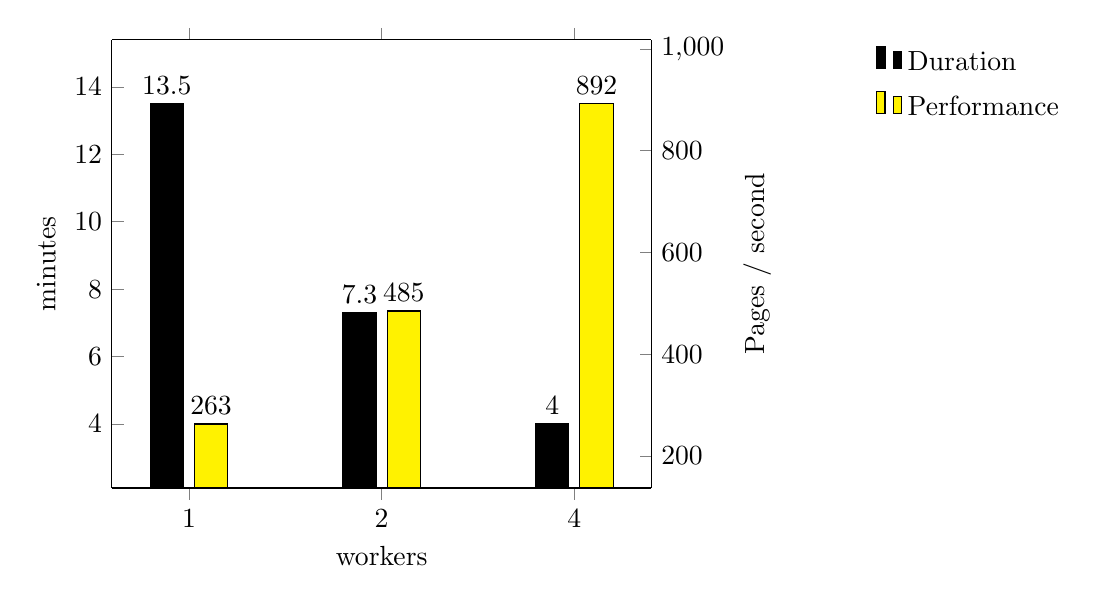
\begin{tikzpicture} 
  \begin{axis}[
    ybar,
    bar width=12pt,
    bar shift=-8pt,
    axis y line*=left,
    enlargelimits=0.2,
    xlabel={workers},
    xlabel near ticks,
    ylabel={minutes},
    ylabel near ticks,
    xtick=data,
    symbolic x coords={1,2,4},
    legend style={at={(1.4,1)}, anchor=north west, draw=none},
    nodes near coords,
    nodes near coords align={vertical},
    ]
    \addplot[fill=black]
      coordinates {(1,13.5) (2,7.3) (4,4.0)};
    \legend{Duration}
  \end{axis}
  \begin{axis}[
    ybar,
    bar width=12pt,
    bar shift=8pt,
    axis y line*=right,
    hide x axis,
    enlargelimits=0.2,
    ylabel={Pages / second},
    ylabel near ticks,
    symbolic x coords={1,2,4},
    legend style={at={(1.4,0.9)},anchor=north west, draw=none},
    nodes near coords,
    nodes near coords align={vertical},
    ]
    \addplot[fill=yellow]
      coordinates {(1,263) (2,485) (4,892)};
  \legend{Performance}
  \end{axis}
\end{tikzpicture}
 
% Chapter Template

\chapter{Conclusions and future work} % Main chapter title
\label{Chapter6} % Change X to a consecutive number; for referencing this chapter elsewhere, use \ref{ChapterX}
\lhead{Chapter 6. \emph{Conclusions and future work}} % Change X to a consecutive number; this is for the header on each page - perhaps a shortened title

Crawl.js is not ready to be let out into the wild. Far from it. It misses many features a mature crawler should have which we discuss in this section. But the focus of Crawl.js was notably to design a distributed crawling architecture able to download sites in parallel and at high speed. An architecture that allows us to crawl sites efficiently and is able to scale easily as needed. Furthermore we wanted an architecture that we can deploy on different (small) data centers in order to be as \emph{close} (in terms of latency) as possible to the sites we fetch. We intentionally left out other important aspects of web crawling such as indexing/searching, page importance, selection policy and revisit policies as many research has been done on those topics already \cite{page_importance1}\cite{page_importance2}\cite{wiki:web_crawler}. Nevertheless, we did design Crawl.js in such a way that features regarding those topics can be added easily some time later.
\newline
\newline
With this in mind we are pretty satisfied with the experiences we gained throughout our work and with the final results we achieved. The Node.js environment proved itself to be a perfect fit for the implementation of Crawl.js. Because of its event-driven model we could keep our code clean and simple. Not only did we never struggle with concurrency-/deadlock situations but the purely asynchronous nature of it granted other advantages:
\begin{itemize}
\item Resource capacity: By tuning the number of concurrent connections we achieved to operate at almost full capacity (~90\% CPU) easily.
\item Good performance: Around 250 pages/second per worker. Especially when taking into account that we parse the downloaded pages too. You find details about the hardware used for one worker in Appendix~\ref{appendix:worker}.
\item Integration with Redis.
\end{itemize}
Working with redis and using its data structures to manage our queues was another great decision we made. The set (sorted-set) structures gave us all the atomic operations we needed and performed very good in our simple experiments. Of course a cluster must be set up as the number of URLs grows to share the key space among multiple servers but for Crawl.js nothing changes if using a cluster or a single server. Furthermore, is the ability of distributing the key space to different servers (data-centers) a feature that the Crawl.js system highly values. Remember we wanted an architecture deployable to different (small) data centers.
\newline
With the help of the set (sorted-set) structures we could also easily introduce groups of workers in order to respect \emph{closeness} to the pages we fetch. Groups (and blocks) are nothing more than (set-)keys of the following form: 'group:XX:block:YY'. And because the redis commands used to manipulate the sets (sorted-sets) are mostly able to deal with multiple values (members) at once, we were able to implement a simple batch processing of URLs very easily. This made the communication between the workers and redis very efficient.
\newline
Last but not least we achieved an almost linear scaling behaviour, which in our eyes is a pretty good foundation to build upon.

\section{Future work}
Here are some ideas how Crawl.js could evolve in the future. They came across during our work and could not be implemented mostly because of time/focus constraints. The order is purely random and has nothing to do with our preference.

\subsection{Dynamic configuration}
In Crawl.js the configuration is done statically. We define the number of groups (and the number of blocks within them) in a file \emph{before} we start the crawler. In our simple experiment setup this was good enough. But the need to this during \emph{runtime} is obvious. Especially when crawling the public internet (or part of) the number of workers needed (to finish in a reasonable time) is not known in advance. Neither how to distribute them to the different groups, or how many groups are needed at all. Therefore a configuration/monitoring channel is really needed. Through this communication channel the workers would \emph{announce} them self and request a valid configuration to start crawling. Of course new configurations could be pushed during runtime too. Additionally monitoring functionalities could go through this channel too which leads us to the next section. 

\subsection{Administration}
Making sure that all workers (and other components) are alive and healthy is a need that becomes more and more important as the number of components within the system grows. As an administrator of the system we need to \emph{monitor} the components and have some sort of an interface to take appropriate \emph{actions}.

\subsection{Blacklist}
The management of a global blacklist is just an example of an important administration task. When crawling the public internet we need to be able to react to the following example situations:
\begin{itemize}
  \item Rescue workers from spider traps \cite{wiki:spider_trap}.
  \item React to complaints about our crawler.
\end{itemize}

\subsection{Public crawl}
We did mention that crawling the public internet would be the next step to really test Crawl.js. In order to do that a good supervision is essential. Especially handling complaints quickly in order not to ruin the reputation of Crawl.js. When designing and implementing a crawler errors such as crawling a site too often are inevitable and therefore a good administration is essential. Therefore we suggest to implement an administration interface \emph{before} doing a significantly big public crawl.

\subsection{URL normalization}
The topic of URL normalization \cite{wiki:url_normalization} was absolutely not respected during our implementation. Future versions of Crawl.js should consider implementing at least the discussed approaches in RFC3986 \cite{rfc:url_normalization}.

\subsection{Page importance}
Page importance and related graph problems have not been taken into account. The order at which Crawl.js fetches pages is random. While the topic of page importance is complex it could be implemented easily in Crawl.js, mainly because Crawl.js uses distributed (sorted-) sets to manage URLs. With this data structure a PageRank\cite{google} could be computed off-line and the resulting sorted set used by the workers. Or maybe a novel on-line algorithm such as OPIC (On-line Page Importance Computation) \cite{page_importance1} could be implemented as well.
 

%----------------------------------------------------------------------------------------
%	THESIS CONTENT - APPENDICES
%----------------------------------------------------------------------------------------

\addtocontents{toc}{\vspace{2em}} % Add a gap in the Contents, for aesthetics

\appendix % Cue to tell LaTeX that the following 'chapters' are Appendices

% Include the appendices of the thesis as separate files from the Appendices folder
% Uncomment the lines as you write the Appendices

% Appendix A

\chapter{Configuration - config.json - Experiment 3} % Main appendix title
\label{appendix:config.json} % For referencing this appendix elsewhere, use \ref{AppendixA}
\lhead{Appendix A. \emph{Configuration - config.json - Experiment 3}} % This is for the header on each page - perhaps a shortened title

Here you find the configuration as used during Experiment 3. More precisely test 3 of experiment 3. It uses a total of 4 workers (10 connections each) assigned to 2 groups. Group 0 having 1 worker and group 1 with 3 workers.
\newline
The format is in JSON.\cite{wiki:json}
\begin{lstlisting}[language=JavaScript]
{
  "group": "the group we are crawling for. defined by argv[1]",
  "block": "the block we are crawling for. defined by argv[2]",
  "mapper": {
    "rules": [
      {"hostname": "bs.wikipedia.org", "group": 0 },
      {"hostname": "bn.wikipedia.org", "group": 1 }
    ],
    "groups": [
      {"group": 0, "blocks": 1},
      {"group": 1, "blocks": 3}
    ]
  },
  "fetcher": {
    "instances": 10,
    "request": {
        "jar": true,
        "timeout": 30000,
        "followRedirect": true,
        "maxRedirects": 3,
        "headers": {
          "User-Agent": "crawl.js v0.0.1"
        }
    }
  },
  "extractor": "parser",
  "queues": {
    "local": {
      "type": "memory",
      "options": {
        "limit": 10000
      }
    },
    "remote": {
      "type": "redis",
      "options": {
        "flushInterval": 10000,
        "host": "redis0",
        "port": "6379"
      }
    }
  },
  "seen": {
    "host": "redis0",
    "port": "6379"
  },
  "dispatcher": {
    "acceptPattern": "http://(bs|bn).wikipedia.org/articles"
  },
  "store": {
    "type": "dummy",
    "options": {}
  },
  "robo": {
    "limit": 100
  }
}
\end{lstlisting}
% Appendix A

\chapter{Worker hardware details (lshw)} % Main appendix title
\label{appendix:worker} % For referencing this appendix elsewhere, use \ref{AppendixA}
\lhead{Appendix A. \emph{Worker hardware details}} % This is for the header on each page - perhaps a shortened title

Thats the output (stripped down) of the command \emph{lshw} from one of our VMs used throughout the experiments. With such hardware we achieved around 250 pages / second.
\newline
\begin{lstlisting}[language=Bash]
sudo lshw -c cpu -c memory -c network
  *-cpu
       description: CPU
       product: QEMU Virtual CPU version 1.0
       vendor: Intel Corp.
       physical id: 401
       bus info: cpu@0
       slot: CPU 1
       size: 2GHz
       capacity: 2GHz
       width: 64 bits
  *-memory
       description: System Memory
       physical id: 1000
       size: 1GiB
       capacity: 1GiB
     *-bank
          description: DIMM RAM
          physical id: 0
          slot: DIMM 0
          size: 1GiB
          width: 64 bits
  *-network
       description: Ethernet interface
       product: RTL-8139/8139C/8139C+
       vendor: Realtek Semiconductor Co., Ltd.
       physical id: 3
       bus info: pci@0000:00:03.0
       logical name: eth0
       version: 20
       serial: 02:00:c0:a8:62:09
       size: 100Mbit/s
       capacity: 100Mbit/s
       width: 32 bits
       clock: 33MHz
  *-memory
       description: RAM memory
       product: Virtio memory balloon
       vendor: Red Hat, Inc
       physical id: 4
       bus info: pci@0000:00:04.0
       version: 00
       width: 32 bits
       clock: 33MHz (30.3ns)
       capabilities: bus_master
       configuration: driver=virtio-pci latency=0
       resources: irq:11 ioport:c120(size=32)
\end{lstlisting}
%\input{./Appendices/AppendixC}

\addtocontents{toc}{\vspace{2em}} % Add a gap in the Contents, for aesthetics

\backmatter

%----------------------------------------------------------------------------------------
%	BIBLIOGRAPHY
%----------------------------------------------------------------------------------------

\label{Bibliography}

\lhead{\emph{Bibliography}} % Change the page header to say "Bibliography"

\bibliographystyle{unsrtnat} % Use the "unsrtnat" BibTeX style for formatting the Bibliography

\bibliography{Bibliography} % The references (bibliography) information are stored in the file named "Bibliography.bib"

\end{document}  